\begin{titre}[Fonctions de référence]

\Titre{Fonctions de référence}{2}
\end{titre}


\subsection*{Matériel et mise en œuvre}

Pour chaque fonction de référence (carré, inverse, racine carrée, cube, affine : définitions et courbes représentatives) :

\begin{description}
 \item[•] Tableau de signes
  \item[•] Tableau de valeurs
 \item[•] Tableau de variations   
  \item[•] Courbe
  \item[•] Définition
 \end{description} 

Les élèves doivent reformer les fonctions de référence.  


\subsection*{Matériel}
 
 
\subsubsection*{Les définitions}


\begin{DefN}
On appelle \emph{fonction Inverse} la fonction définie sur $\mathbb{R}^*=]-\infty;0[\cup]0;+\infty[$ par $f : x\mapsto \dfrac{1}{x}$ ou $f(x)=\dfrac{1}{x}$.
\end{DefN}

\vspace{0.4cm}

\begin{DefN}
On appelle \emph{fonction Carré} la fonction définie sur $\mathbb{R}=]-\infty;+\infty[$ par $f : x\mapsto  x^2$ ou $f(x)=x^2$. 
\end{DefN}

\vspace{0.4cm} 

\begin{DefN}
On appelle \emph{fonction Cube} la fonction définie sur $\mathbb{R}=]-\infty;+\infty[$ par $f : x\mapsto  x^3$ ou $f(x)=x^3$. 
\end{DefN}

\vspace{0.4cm} 

\begin{DefN}
On appelle \emph{fonction Racine Carrée} la fonction définie sur $\mathbb{R^+}=[0;+\infty[$ par $f : x\mapsto  \sqrt{x}$ ou $f(x)=\sqrt{x}$. 
\end{DefN}

\vspace{0.4cm} 

\begin{DefN}
On appelle \emph{fonction affine} la fonction définie sur $\mathbb{R}=]-\infty;+\infty[$ par $f(x)=  ax+b$. 
\end{DefN} 

 \newpage
 
\subsubsection*{Les tableaux de signes} 

 \begin{tikzpicture}
   \tkzTabInit{$x$ / 1 , $f(x)$ / 1}{$-\infty$, $x_0$, $+\infty$}
   \tkzTabLine{,$-$, z, $+$, }
\end{tikzpicture}


\vspace{0.4cm}

\begin{tikzpicture}
   \tkzTabInit{$x$ / 1 , $f(x)$ / 1}{$-\infty$, $0$, $+\infty$}
   \tkzTabLine{,$+$, z, $+$, }
\end{tikzpicture}

\vspace{0.4cm}

\begin{tikzpicture}
   \tkzTabInit{$x$ / 1 , $f(x)$ / 1}{$-\infty$, $0$, $+\infty$}
   \tkzTabLine{,$-$, z, $+$, }
\end{tikzpicture}
\vspace{0.4cm}

\begin{tikzpicture}
   \tkzTabInit{$x$ / 1 , $f(x)$ / 1}{$-\infty$, $-2$, $+\infty$}
   \tkzTabLine{,$-$, z, $+$, }
\end{tikzpicture}

\vspace{0.4cm}

\begin{tikzpicture}
   \tkzTabInit{$x$ / 1 , $f(x)$ / 1}{$-\infty$, $0$, $+\infty$}
   \tkzTabLine{,$-$, d, $+$, }
\end{tikzpicture}

\vspace{0.4cm}

\begin{tikzpicture}
   \tkzTabInit{$x$ / 1 , $f(x)$ / 1}{$-\infty$, $0$, $+\infty$}
   \tkzTabLine{,$+$, d, $+$, }
\end{tikzpicture}

\vspace{0.4cm}

\begin{tikzpicture}
   \tkzTabInit{$x$ / 1 , $f(x)$ / 1}{$-\infty$, $0$, $+\infty$}
   \tkzTabLine{,$-$, z, $+$, }
\end{tikzpicture}

\vspace{0.4cm}

\begin{tikzpicture}
   \tkzTabInit{$x$ / 1 , $f(x)$ / 1}{  $0$, $+\infty$}
   \tkzTabLine{$0$,   $+$, }
\end{tikzpicture}

\vspace{0.4cm}

\begin{tikzpicture}
   \tkzTabInit{$x$ / 1 , $f(x)$ / 1}{  $0$, $+\infty$}
   \tkzTabLine{$0$,   $-$, }
\end{tikzpicture}
 \newpage
 
\subsubsection*{Les tableaux de valeurs} 

\begin{tabular}{|c|c|c|c|c|c|c|c|}
\hline 
$x$ & 0 & $\frac{1}{4}$ & 1 & 2,25 & 4 & 9 \\ 
\hline 
$f(x)$ & 0 & 0,5  & 1 & 1,5  & 2 & 3\\ 
\hline 
\end{tabular} 

\vspace{0.4cm}

\begin{tabular}{|c|c|c|c|c|c|c|c|c|c|c|c|c|c|c|c|}
\hline 
$x$ & $-3$ & $-\frac{5}{2}$ & $-2$ & $-\frac{3}{2}$ & $-1$ & $-0,5$ &  0 & $\frac{1}{2}$ & 1 & $\frac{3}{2}$ & 2 & 2,5 & 3 \\ 
\hline 
$f(x)$ & 9 & 6,25 & 4 & 2,25 & 1 & $\frac{1}{4}$ & 0 & 0,25 & 1 & 2,25 & 4 & 6,25 & 9 \\ 
\hline 
\end{tabular} 

\vspace{0.4cm}

\begin{tabular}{|c|c|c|c|c|c|c|c|c|c|c|c|c|c|c|c|}
\hline 
$x$ & $-3$ & $-\frac{5}{2}$ & $-2$ & $-\frac{3}{2}$ & $-1$ & $-0,5$ &  0 & $\frac{1}{2}$ & 1 & $\frac{3}{2}$ & 2 & 2,5 & 3 \\ 
\hline 
$f(x)$ & $-27$ & $-15,625$ & $-8$ & $-3,375$ & 1 & $\frac{1}{8}$ & 0 & 0,125 & 1 & 3,375 & 8 & 15,625  & 27 \\ 
\hline 
\end{tabular} 

\vspace{0.4cm}

\begin{tabular}{|c|c|c|c|c|c|c|c|c|c|c|c|c|c|c|c|}
\hline 
$x$ & $-5$ & $-4$ & $-2$ &   $-1$ & $-0,5$ &  0 & $\frac{1}{2}$ & 1 & 2 &   4 & 5 \\ 
\hline 
$f(x)$ & $-\frac{1}{5}$ & $-0,25$ &   $-0,5$ & $-1$ & $-0,2$ & 0 & 0,2  & 1 & 0,5 &  0,25  & 0,2 \\ 
\hline 
\end{tabular}

\vspace{0.4cm}

\begin{tabular}{|c|c|c|c|c|c|c|c|c|c|c|c|c|c|c|c|}
\hline 
$x$ & $-5$ & $-4$ & $-2$ &   $-1$ & $-0,5$ &  0 & $\frac{1}{2}$ & 1 & 2 &   4 & 5 \\ 
\hline 
$f(x)$ & $-\frac{1}{5}$ & $-0,25$ &   $-0,5$ & $-1$ & $-2$ & 0 & 2 & 1 & 0,5 &  0,25  & 0,2 \\ 
\hline 
\end{tabular}

\vspace{0.4cm} 

\begin{tabular}{|c|c|c|c|c|c|c|c|c|c|c|c|c|c|c|c|}
\hline 
$x$ & $-10$ &   $-5$ &  0 & 5 & 10 \\ 
\hline 
$f(x)$ & $-1$ &   $0$ &  1 & 2 & 3  \\ 
\hline 
\end{tabular}


\subsubsection*{Propriétés des variations} 

\begin{ThN}
La fonction \emph{Cube} est strictement croissante sur $\R$. 
\end{ThN}

\vspace{0.4cm} 

\begin{ThN}
La fonction \emph{Inverse} est décroissante sur $]-\infty;0[$ et  décroissante sur $]0;+\infty[$. 
\end{ThN}

\vspace{0.4cm}

\begin{ThN}
La fonction \emph{Carré} est strictement décroissante sur $\R^-$ et strictement croissante sur $\R^+$. 
\end{ThN}

\vspace{0.4cm} 

\begin{ThN}
La fonction \emph{Racine Carrée} est strictement croissante sur $\R+$. 
\end{ThN}

\vspace{0.4cm} 
 
 \begin{ThN}
La fonction \emph{affine}, $f:x \mapsto ax +b$ définie sur $\R$, est strictement croissante sur $\R$ lorsque $a>0$, strictement décroissante sur $\R$ lorsque $a<0$. 
\end{ThN}

 \newpage
 
\subsubsection*{Les tableaux de variations} 

\begin{tikzpicture}
   \tkzTabInit{$x$ / 1 , $f(x)$ / 2}{$-\infty$,   $+\infty$}
   \tkzTabVar{+/ $+\infty$, -/ $-\infty$}
\end{tikzpicture}



\vspace{0.4cm}

\begin{tikzpicture}
   \tkzTabInit{$x$ / 1 , $f(x)$ / 2}{$-\infty$,   $+\infty$}
   \tkzTabVar{-/ $+\infty$, +/ $-\infty$}
\end{tikzpicture}



\vspace{0.4cm}

\begin{tikzpicture}
   \tkzTabInit{$x$ / 1 , $f(x)$ / 2}{$-\infty$,   $+\infty$}
   \tkzTabVar{-/ $-\infty$, +/ $+\infty$}
\end{tikzpicture}

\vspace{0.4cm}

\begin{tikzpicture}
   \tkzTabInit{$x$ / 1 , $f(x)$ / 2}{$-\infty$, 0 ,  $+\infty$}
   \tkzTabVar{-/ $+\infty$,  +/0 ,  -/ $+\infty$}
\end{tikzpicture}

\vspace{0.4cm}

\begin{tikzpicture}
   \tkzTabInit{$x$ / 1 , $f(x)$ / 2}{$-\infty$, 0 ,  $+\infty$}
   \tkzTabVar{+/ $+\infty$,  -/0 ,  +/ $+\infty$}
\end{tikzpicture}

\vspace{0.4cm}

\begin{tikzpicture}
\tkzTabInit[lgt=1,espcl=2]{ $x$ / 1,$f $ / 2}
{ $-\infty$ , $0$ ,$+\infty$}
\tkzTabVar{+/$0$ , -D+ /$ $/$ $ , -/$0$}
\end{tikzpicture}
\vspace{0.4cm}

\begin{tikzpicture}
   \tkzTabInit{$x$ / 1 , $f(x)$ / 2}{$-\infty$,   $+\infty$}
   \tkzTabVar{-/ $-\infty$, +/ $+\infty$}
\end{tikzpicture}

\vspace{0.4cm}

\begin{tikzpicture}
   \tkzTabInit{$x$ / 1 , $f(x)$ / 2}{0,   $+\infty$}
   \tkzTabVar{-/ $-\infty$, +/ $+\infty$}
\end{tikzpicture}

  

 
 
 
 
 
 
\subsubsection*{Les courbes}

\begin{tikzpicture}[line cap=round,line join=round,>=triangle 45,x=1.0cm,y=1.0cm]
\begin{axis}[
x=1.0cm,y=1.0cm,
axis lines=middle,
ymajorgrids=true,
xmajorgrids=true,
xmin=-7.66,
xmax=4.12,
ymin=-2.38,
ymax=2.7,
xtick={-7.0,-6.0,...,4.0},
ytick={-2.0,-1.0,...,2.0},]
\clip(-7.66,-2.38) rectangle (4.12,2.7);
\draw [line width=2.pt,domain=-7.66:4.12] plot(\x,{(--1.--0.2*\x)/1.});
\end{axis}
\end{tikzpicture}



\begin{tikzpicture}[line cap=round,line join=round,>=triangle 45,x=1.0cm,y=1.0cm]
\begin{axis}[
x=1.0cm,y=1.0cm,
axis lines=middle,
ymajorgrids=true,
xmajorgrids=true,
xmin=-2.98,
xmax=3.54,
ymin=-0.8999999999999996,
ymax=6.659999999999997,
xtick={-2.0,-1.0,...,3.0},
ytick={-0.0,1.0,...,6.0},]
\clip(-2.98,-0.9) rectangle (3.54,6.66);
\draw [samples=50,rotate around={0.:(0.,0.)},xshift=0.cm,yshift=0.cm,line width=2.pt,domain=-4.0:4.0)] plot (\x,{(\x)^2/2/0.5});
\end{axis}
\end{tikzpicture}

 
\begin{tikzpicture}[line cap=round,line join=round,>=triangle 45,x=1.0cm,y=1.0cm]
\begin{axis}[
x=1.0cm,y=1.0cm,
axis lines=middle,
ymajorgrids=true,
xmajorgrids=true,
xmin=-0.640000000000001,
xmax=9.520000000000007,
ymin=-0.6600000000000019,
ymax=4.239999999999996,
xtick={-0.0,1.0,...,9.0},
ytick={-0.0,1.0,...,4.0},]
\clip(-0.64,-0.66) rectangle (9.52,4.24);
\draw[line width=2.pt,color=black,smooth,samples=100,domain=4.079999953157344E-8:9.520000000000007] plot(\x,{sqrt((\x))});
\end{axis}
\end{tikzpicture}


 
\begin{center}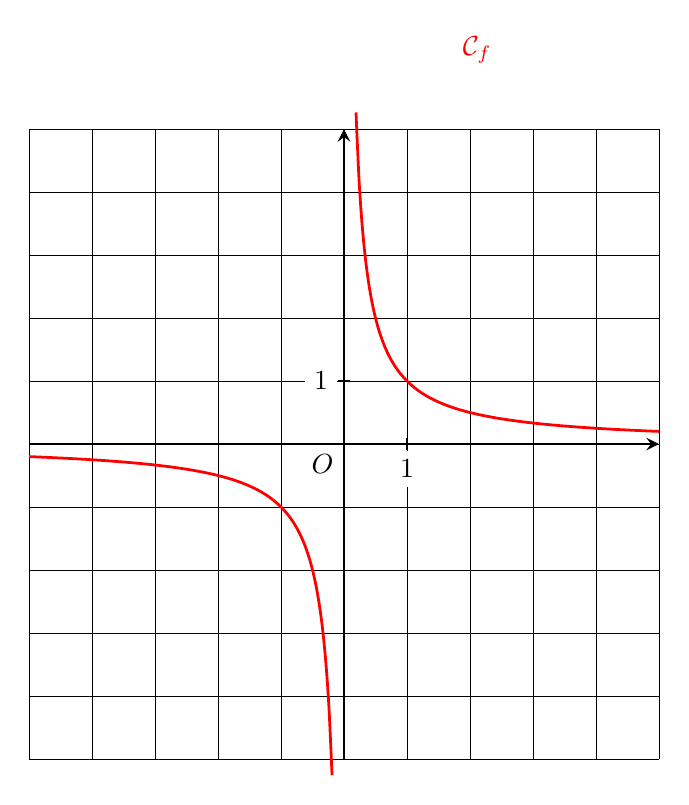
\begin{tikzpicture}[x=.8cm,y=.8cm,>=stealth]
\draw[line width=.1pt] (-5,-5) grid[step=1] (5,5);
\draw[line width=1pt] (0,0) node[below left, fill=white]{$O$} (1,-2pt) node[below, fill=white]{$1$} --(1,2pt) (-2pt,1) node[left, fill=white]{$1$} --(2pt,1);
\draw[color=red] (2.5,6.25) node[left,fill=white]{$\mathcal{C}_f$};
\draw[line width=1pt,->] (-5,0)--(5,0);
\draw[line width=1pt,->] (0,-5)--(0,5);
\draw[line width=1pt,color=red] plot[smooth, samples=100, domain=-5:-0.19] (\x,{1/\x});
\draw[line width=1pt,color=red] plot[smooth, samples=100, domain=0.19:5] (\x,{1/\x});
\end{tikzpicture}\end{center}


 
\begin{tikzpicture}[line cap=round,line join=round,>=triangle 45,x=1.0cm,y=0.38800705467372043cm]
\begin{axis}[
x=1.0cm,y=0.38800705467372043cm,
axis lines=middle,
ymajorgrids=true,
xmajorgrids=true,
xmin=-2.896551724137932,
xmax=2.8965517241379306,
ymin=-10.09090909090913,
ymax=15.681818181818203,
xtick={-2.0,-1.0,...,2.0},
ytick={-10.0,-5.0,...,15.0},]
\clip(-2.896551724137932,-10.09090909090913) rectangle (2.8965517241379306,15.681818181818203);
\draw[line width=2.pt,color=black,smooth,samples=100,domain=-2.896551724137932:2.8965517241379306] plot(\x,{(\x)^(3.0)});
 
\end{axis}
\end{tikzpicture}



